\section{Højtaleren i Basrefleks-kabinet}

For at kunne sammenligne teori og praksis, kan højtaler-dataen fra tabel \ref{tab:TS} benyttes til at udformere et simuleret frekvensrespons, for de forskellige portlængder på basrefleksen.

Ved at beregne volumenhastigheden for den elektriske impedans, ud fra teorien behandlet i afsnit \ref{chapt:Teori}, kan man opdele bidraget fra fronten af højtaleren og for porten, for til sidst at lave det samlede lydtryk til en ønsket afstand \textit{r}. 


%\subsection{Volumenhastighed Front:}
%\label{sec:sim_calc}

%Ud fra impedansen af det samlede system, kan volumenhastigheden for højtalerenheden i kabinettet beregnes. Dette er hastigheden af det volumen af luft som skubbes foran højtaleren. 

%<<<<<<< HEAD
%{\large\(qF=\)}{\Large \(\frac{F_A}{R_{AE}+s*M_{AS}+\frac{1}{s*C_{AS}}+Ras+\frac{1}{(s*C_{AB}+\frac{1}{s*M_{AP}}}}\) }
%=======
%\begin{equation}
%	qF=\frac{F_A}{R_{AE}+s*M_{AS}+\frac{1}{s*C_{AS}}+Ras+\frac{1}{s*C_{AB}+\frac{1}{s*M_{AP}}} }
%\end{equation}

%>>>>>>> 1ddbb399d9df3a1dd1363b7c180a1e0b12ec412c


%Hvor\\

%\(M_{AP}=\frac{(\rho)}{S_P}*(L_P+1.46*\sqrt{\frac{S_P}{\pi}}\)  \hspace{3.1 cm} Luftmassen i den Akustiske Port\\

%Det ses her, at $M_{AP}$ er afhængig af længden på porten $L_P$. For at opnå en korrekt afstemning af porten ift. højtalerenhedens resonansfrekvens, beregnes denne portlængde som følger:

%\(r_P=0.025 m\)		\hspace{6.2cm} Portens Radius\\
%\(S_P=\pi*r_P^2=pi*0.025^2=0.0020 m^2\)		%\hspace{2cm} Portens overfladeareal\\
%\(L_P=\frac{\gamma*P_0}{\rho*(2*\pi*f_p)^2*V_{B}}-1.46\sqrt{\frac{S_P}{\pi}}\)			\hspace{3cm} Længden på porten\\

%$\gamma \approx 1.4$ \& $P_0=100*10^3)$\\

%Dermed får vi den optimale portlængde:\\

%\(L_P=\frac{1.4*100*10^3}{1.18*(2*\pi*44)^2*16.5*10-3}-1.46\sqrt{\frac{0.0020}{\pi}}=15cm\)


%\subsection{Volumenhastighed Port:}

%<<<<<<< HEAD
%Tilsvarende beregnes bidraget fra porten ud fra følgende formel:

%{\large\(qP=-qF*\)}{\Large \(\frac{\frac{1}{s*C_{AB}}}{\frac{1}{s*C_{AB}}+s*M_{AP}}\) }
%\cite{Elektroakustik}
%=======
%Tilsvarende beregnes bidraget fra porten ud fra følgende formel \ref{lign:qP}:
%\begin{equation}\label{lign:qP}
%	qP=-qF* \frac{\frac{1}{s*C_{AB}}}{\frac{1}{s*C_{AB}}+s*M_{AP}} 	
%\end{equation}

%>>>>>>> 1ddbb399d9df3a1dd1363b7c180a1e0b12ec412c


%\subsection{Beregning af samlet lydtryk:}

%<<<<<<< HEAD
%For at omregne de to volumenhastigheder til et lydtryk i afstanden \textit{r} med enheden dB SPL, benyttes følgende formel:

%\(L=20*log_{10}(\frac{\frac{\rho*f}{r}*(qF+qP)}{pRef}) dB SPL\)

%hvor referencetrykket $pRef=10  \mu Pa$
%=======
%For at omregne de to volumenhastigheder til et lydtryk i afstanden \textit{r} med enheden dB SPL, benyttes følgende formel \ref{lign:L}:

%\begin{equation}\label{lign:L}
%	L=20*log_{10}(\frac{\frac{\rho*f}{r}*(qF+qP)}{pRef}) dB SPL
%\end{equation}

%hvor referencetrykket $pRef=20  \mu Pa$
%>>>>>>> 1ddbb399d9df3a1dd1363b7c180a1e0b12ec412c


\subsection{Resultater}

Ved beregningen i Matlab, kan der simuleres et plot for frekvenskarakteristikken af bidraget fra højtalerenheden, porten og det samlede bidrag. \\
For at eftervise at det 14cm lange rør er den optimale længde for basreflexen i projektets kabinet, er der ligeledes lavet simuleringer med de to andre test-størrelser som var fysisk til rådighed: 7cm og 3.5cm.

\subsubsection{Kort port - 3.5 cm}

Ved brug af en portlængde på 3.5 cm, fås frekvensresponset som ses på figur \ref{fig:sim_kort}. \\
Det fremgår af figuren at portens resonansfrekvens fp er helt oppe på 71 Hz, hvilket er over 2/3 højere end højtalerennhedens resonans. Dermed er porten ikke ordentligt afstemt, og de 24dB/oktav's fald under fp koster betydeligt på de lavere frekvenser. 

\begin{figure}[h!]
	\centering
	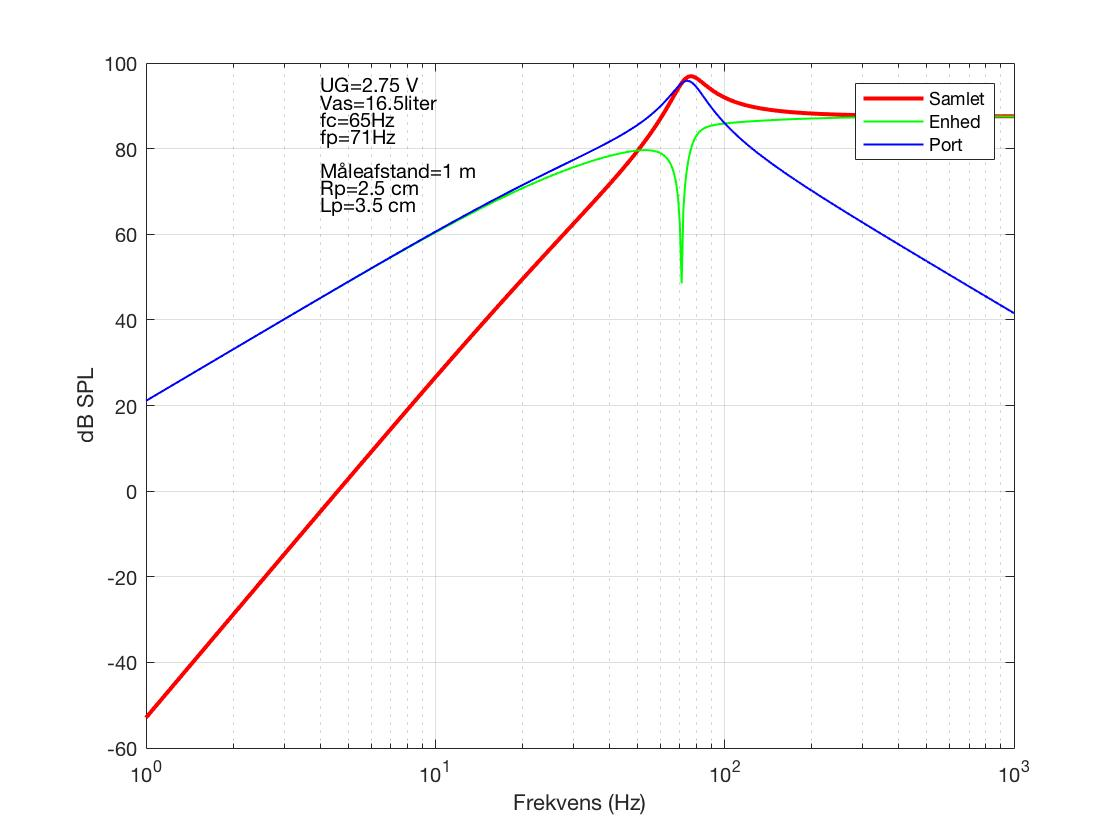
\includegraphics[width=.75\textwidth]{Pics/sim_kort}
	\caption{Simuleret frekvensrespons ved $L_P$=3.5cm } 
	\label{fig:sim_kort}
\end{figure}

\subsubsection{Mellemlangt port - 7 cm}

Ved brug af en portlængde på 7 cm, fås frekvensresponset som ses på figur \ref{fig:sim_medium}. \\
Det ses nu, at portens resonansfrekvens er rykket længere ned og nu resonerer ved 58 Hz. Dette er væsentligt tættere på at være afstemt med højtalerenhedens opgivne 45 Hz resonans, men er endnu ikke nede og give et korrekt bidrag for at løfte de lavere frekvenser. 

Det er ligeledes værd at notere, at det generelle gain som er opnået, er lavere for den mellemlange port end for den korte port.  

\begin{figure}[h!]
	\centering
	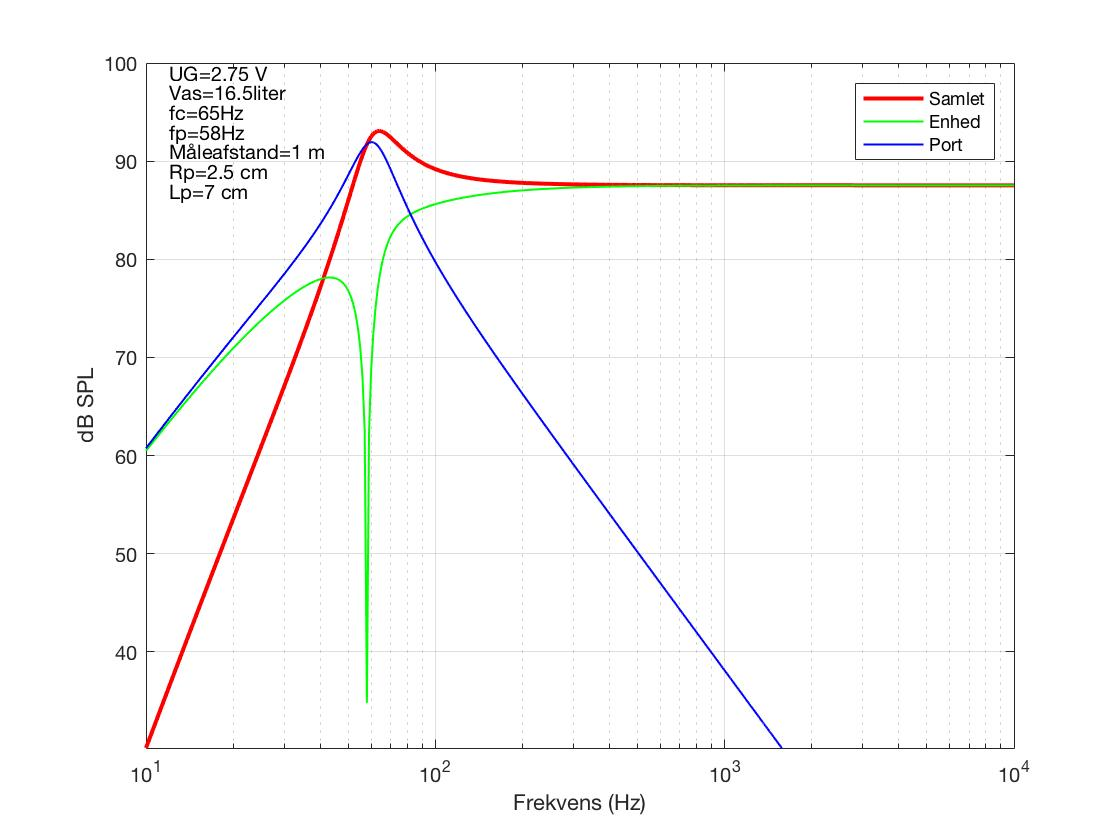
\includegraphics[width=.75\textwidth]{Pics/sim_medium}
	\caption{Simuleret frekvensrespons ved $L_P$=7cm } 
	\label{fig:sim_medium}
\end{figure}

\subsubsection{Langt port - 14 cm}

Ved brug af en portlængde på 14 cm, fås frekvensresponset som ses på figur \ref{fig:sim_langt}. \\
Denne længde er den teoretisk optimale, som det blev beregnet ovenfor i sektion \ref{sec:theori_calc}, og resonerer nu i 44 Hz, så port og højtaler er korrekt afstemt. 
Der opretholdes dermed en højere gengivelse af de lavere frekvenser end det var muligt før og teorien stammer dermed overens med simuleringen. 

\begin{figure}[h!]
	\centering
	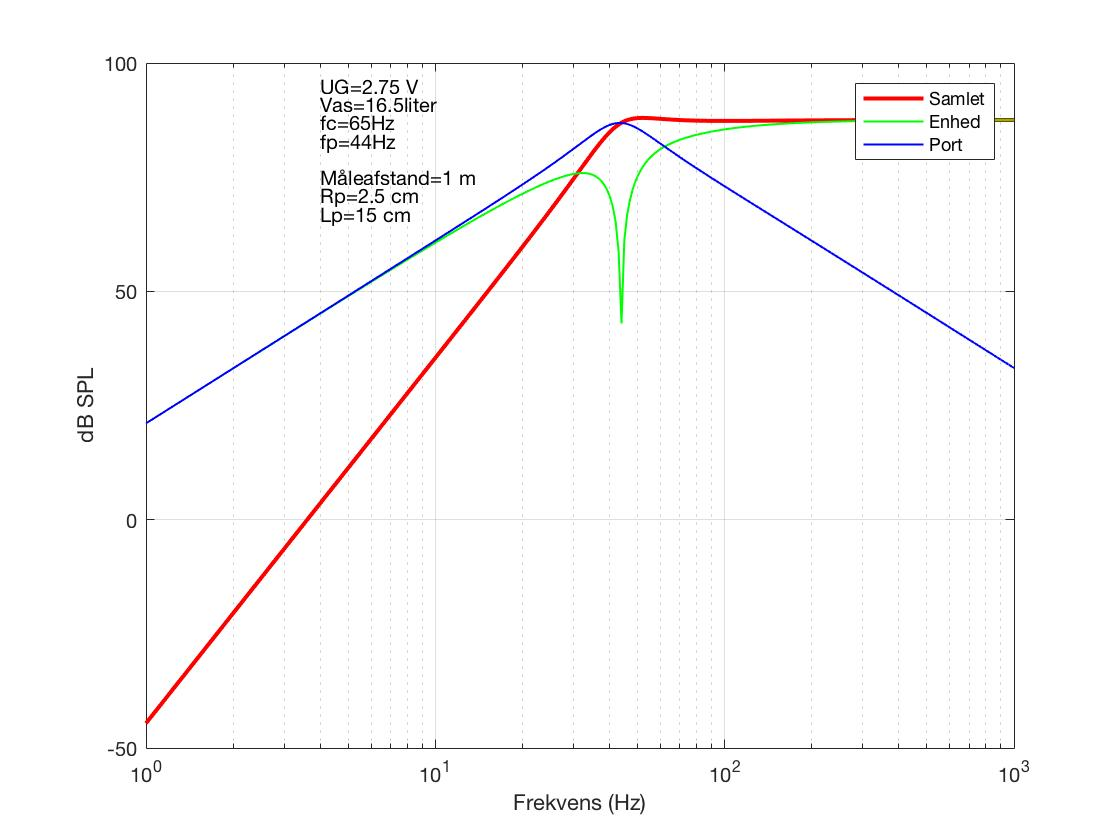
\includegraphics[width=.75\textwidth]{Pics/sim_lang}
	\caption{Simuleret frekvensrespons ved $L_P$=14cm } 
	\label{fig:sim_langt}
\end{figure}

Det kan ydermere betragtes, at kurven aftager med 24dB/oktav under højtalerens resonansfrekvens, netop som teorien beskrev.\cite{Elektroakustik}

\section{Bidrag fra reflektion}
\label{sec:reflection}
Foruden at skabe den bedst mulige gengivelse af de laveste frekvenser muligt vha. et afstemt basreflex-kabinet, fokuserer dette projekt på at forsøge at skabe et yderligere bidrag i bassen ved hjælp af et refleksionsbidrag fra nærliggende overflader. 

Teorien beror sig på et fokus for refleksion ved en højtaler placeret i en vis højde fra gulvet. Her tages der dog ikke forbehold for kabinet-typen, betydende at positionen af basrefleks-porten heller ikke tages i betragtning. 
Dette er dog et fokuspunkt for målingen, hvor simuleringen alene anvender den teori som er afbilledet i bogen (figur \ref{fig:reflect}
\cite{Elektroakustik}


\begin{figure}[h!]
	\centering
	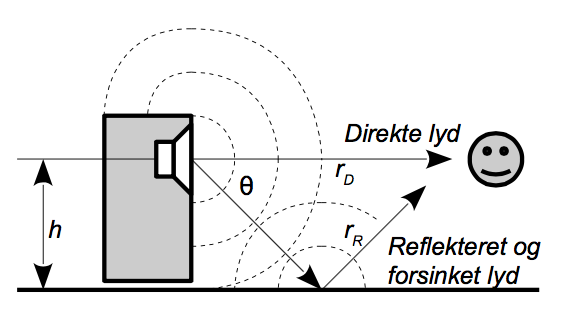
\includegraphics[width=.4\textwidth]{Pics/reflect}
	\caption{Afbilding af teorien bag reflekteret lyd \cite{Elektroakustik} } 
	\label{fig:reflect}
\end{figure}

I jagten på et positivt bidrag i de lave frekvenser, vil man dog kunne forvente en destuktiv interferens, når højtaleren har en afstand til den reflekterede overflade på en halv bølgelængde. Herefter, vil frekvensresponset være temmeligt irregulært, før disse forstyrrelser dør ud i takt med at direktiviteten bliver mere betydende ved høje frekvenser. Dette trade-off skal man kunne leve med, for at refleksionsbidraget vil give mening som en tilstræbelig faktor.\\

Denne frekvens \textbf{$f_R$}, også beskrevet som det første minimum, beregnes ved:\\
\begin{equation}\label{lign:fR}
	f_R=\frac{c}{2(r_R-r_D)}
\end{equation}

hvor $r_R$ er den reflekterede længde, givet ved:
\begin{equation}
	r_R=\sqrt{r_D^2+4h^2}
\end{equation}


Ved højtalerens øgede højder fra gulvet, kan det ses på figur \ref{fig:refleksionsbidrag} at frekvensen for det første minimum falder længere og længere ned. Så ud fra den simple betragtning af denne figur, kan det konkluderes at det må give det højeste stabile bidrag, op imod de højeste frekvenser, ved at sætte højtaleren så tæt på den reflektive overflade som muligt.

\begin{figure}[h!]
	\centering
	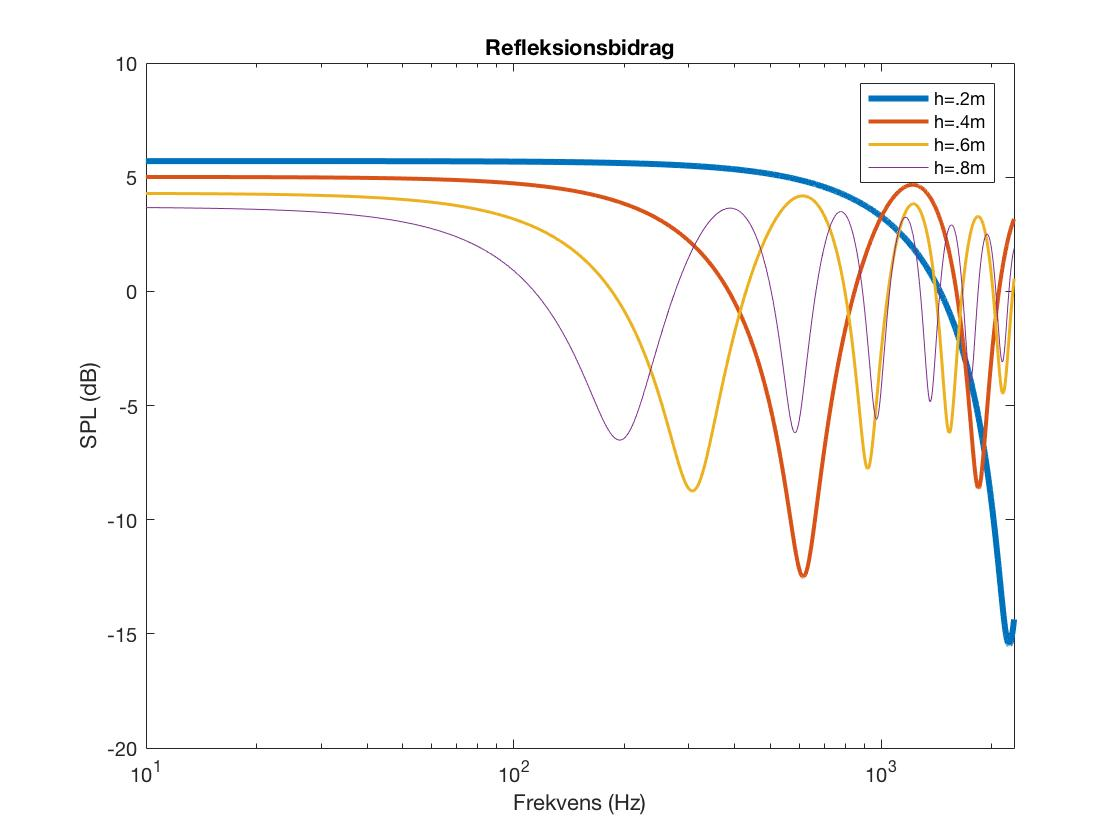
\includegraphics[width=\textwidth]{Pics/refleksionsbidrag}
	\caption{Refleksionsbidrag fra nærmeste hårde, reflekterende overflade til forskellige højder for højtaleren } 
	\label{fig:refleksionsbidrag}
\end{figure}




\section{Samlet Frekvensrespons}

Ved at kombinere bas-reflex kabinettets frekvensrespons med refleksionsbidraget opnås et frekvensrespons som kan ses i figur \ref{fig:sim_samletrespons}.

Af figuren fremgår det, at der er skabt et stabilt gain omkring 6dB i de lavere frekvenser under højtalerens resonansfrekvens, som bringer tidligere uhørbare frekvenser op i et lydtryk, hvor de rent faktisk kan opfattes af det menneskelige ører. Derudover, er de frekvenser som tidligere lå lige på grænsen af denne hørbarhed, løftet til et niveau hvor det burde være væsentligt lettere at høre, hvis man jævnfører med figur \ref{fig:SPL}.

Prisen der betales, er den destuktive interferens som skabes fra reflektionen, set på den blå kurve i figur \ref{fig:sim_samletrespons}, tidligere omtalt i afsnit \ref{sec:reflection}.\\
Dette er trade-off'et imellem forstærkningen i de lave frekvenser og irregulariteten i de højere frekvenser. 

\begin{figure}[h!]
	\centering
	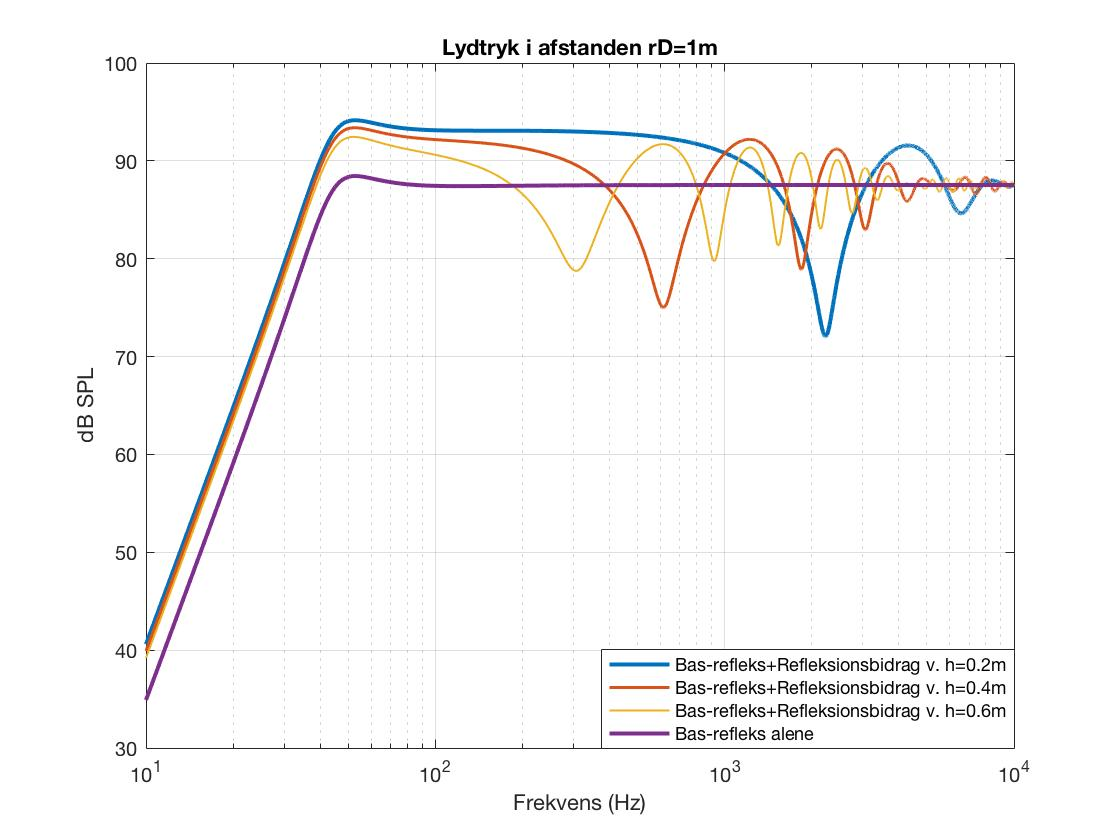
\includegraphics[width=.8\textwidth]{Pics/sim_samletrespons2}
	\caption{Frekvensrespons for Basreflex-kabinettet med vs uden refleksionsbidraget} 
	\label{fig:sim_samletrespons}
\end{figure}

